\chapter{\Rt{} transit data}
\label{cha:data}

\begin{knitrout}\small
\definecolor{shadecolor}{rgb}{0.969, 0.969, 0.969}\color{fgcolor}\begin{kframe}


{\ttfamily\noindent\itshape\color{messagecolor}{\#\# Loading required namespace: transitr}}\end{kframe}
\end{knitrout}

\AT{} operates a fleet of vehicles---including buses, trains, and ferries---to transport passengers around Auckland, New Zealand's largest urban region, from Wellford in the north to Pukekohe in the south \citep{cn}. Serving the region are 1040~routes\footnote{As of 12 August 2019, sourced from \url{https://at.govt.nz/}.}, each providing a service from an \emph{origin} to a \emph{destination} via a specified sequence of \emph{stops} at which passengers may board or alight.


For each route, one or more \emph{trips} are scheduled to operate, typically departing from the origin stop at a fixed time, with approximate arrival times for the intermediate stops along the way. In some cases, services wait at specific stops until the scheduled departure time, known as a \emph{layover}; in others, drivers may adjust their speed to adhere to the schedule. In most cases, however, drivers heed no attention to the schedule and simply drive along the route at whatever speed is reasonable\footnote{At least, this is the case in Auckland.}. Not all trips run every day; typically trips are scheduled as weekday, Saturday, or Sunday and public holidays. Altogther there are (at the time of writing) 24,919~trips provided by \AT{}, 14,022 of which run every weekday.


The assignment of routes, trips, and stops is a common occurence in transport systems, to the extent that it was formalised by Google's \emph{\acrfull{gtfs}} \citep {GoogleDevelopers_2006}. \GTFS{} provides a detailed specification of how transit data should be organised, making it significantly easier for external systems to access, with the primary example being Google Maps, although plenty of other applications exist that make use of it\footnote{Including the one we are presenting.}. \GTFS{} has now been adopted by 1,234~providers across 672~locations globally, which are shown in \cref{fig:gtfs_feeds}. \GTFS{} is discussed further in \cref{sec:gtfs}.

\begin{figure}
\centering
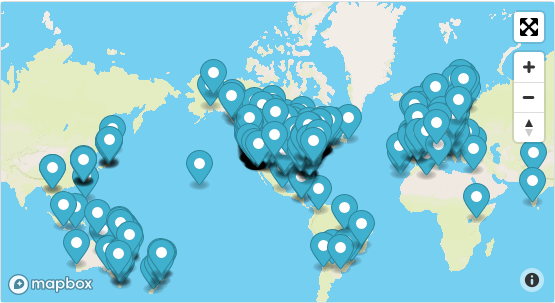
\includegraphics[width=0.8\textwidth]{figure/gtfs_feeds.png}
\caption[Locations of GTFS feed providers]{Locations of the 672~\GTFS{} feed providers,\\
sourced from \url{http://transitfeeds.com/} on 12 Feb 2020.}
\label{fig:gtfs_feeds}
\end{figure}


The vehicles servicing the trips are observed as they travel along the route, either as intermittent \GPS{} locations (\emph{vehicle positions}), or on arrival at or departure from bus stops along the way (\emph{trip updates}). How this data is structured is also specified by \GTFS, and will be described in detail in \cref{sec:realtime-data}, along with a discussion of the issues we encoutered using the \AT{} data.


One of the main ideas we discussed in \cref{sec:literature} was the importance of combining data from multiple routes when predicting arrival times. As it stands, there is no direct method for determining if two routes overlap---that is, share a common path---from \GTFS{} data. The simplest approach would be to compare subsequences of stops, with routes servicing the same stops most likely following the same path between them, although there are several situations where this is not the case. We formalise this idea, as well as expand on it, in \cref{sec:route-segments}.


The \rt{} nature of the application demands predictions be made as soon after observing the data as possible. For this reason, \glspl{rbm} are a logical choice for estimating states in \rt{}, and as such has been used extensively (refer back to \cref{sec:literature}). This family of models are commonly used in vehicle tracking applications, allowing the vehicle's state (such as speed) to be estimated from a \rt{} sequence of noisy measurements of its location. The final section of this chapter provides an introduction to the \glspl{rbm} used throughout the remainder of this thesis.


\section{GTFS}
\label{sec:gtfs}

\glsresetall\phantom{\gls{gps}}

The adoption of GTFS \citep{GoogleDevelopers_2006} by public transport agencies around the world has made it possible for applications such as Google Maps to access and display public transport data to users, regardless of their location. The main goal of GTFS is to specify, in detail, how transit data should be organised so that it is consistent across agencies around the world. As a result, it does not matter whether you are in Auckland, Paris, or C\'ordoba; Google Maps can show you public transport directions by accessing local \gls{gtfs} data.


\GTFS{} consists of two components, \emph{static} and \emph{real-time}.\footnote{The official name is `GTFS-realtime'.} The static component specifies how information about the schedule, fares, and route geographies are organised, while the \emph{real-time} component specifies the format for real-time data: vehicle locations, stop updates and \glspl{eta}, and service advisories. Each of the static and real-time components is implemented by the transit provider; for example, \AT{}'s \GTFS{} service is hosted at \mbox{\url{https://dev-portal.at.govt.nz}}.


\subsection{Static GTFS}
\label{sec:gtfs_static}


\begin{table}[t]
\centering
\fontsize{10}{12}\selectfont
\begin{tabular}{ll}
\toprule
Term & Definition \\
\midrule
route & a collection of \emph{trips} that are displayed to comuters
as a single service \\
trip & a journey servicing two or more stops at a specific time \\
stop & a location where passengers are picked up or dropped off \\
stop time & the (scheduled) times at which vehicles
will arrive at stops for each trip \\
shape & the GPS track a vehicle will take for a specific route \\
\bottomrule
\end{tabular}
\caption[Definitions of GTFS terms]{Definitions of the relevant GTFS terms from \url{https://developers.google.com/transit/gtfs/reference/}}
\label{tab:gtfs_terms}
\end{table}


There are several components of GTFS that are of particular interest to us: routes, trips, stops, stop times, and shapes. The definitions of these terms are given in \cref{tab:gtfs_terms} and \cref{app:gtfs}. Extensive documentation can be found on the GTFS website.\footnote{\url{https://developers.google.com/transit/gtfs/}}


\Cref{fig:gtfs_nw} demonstrates a single \emph{route} along which there are two active \emph{trips} (A and B). The route's \emph{shape} is represented by the line connecting the six \emph{stops} numbered 1--6. The real-time arrivals board or \gls{dms} is shown for stop~5, displaying the scheduled \emph{stop time} (arrival time) for each trip at that stop. The additional information displayed is described in the next section.



\begin{knitrout}\small
\definecolor{shadecolor}{rgb}{0.969, 0.969, 0.969}\color{fgcolor}\begin{figure}

{\centering 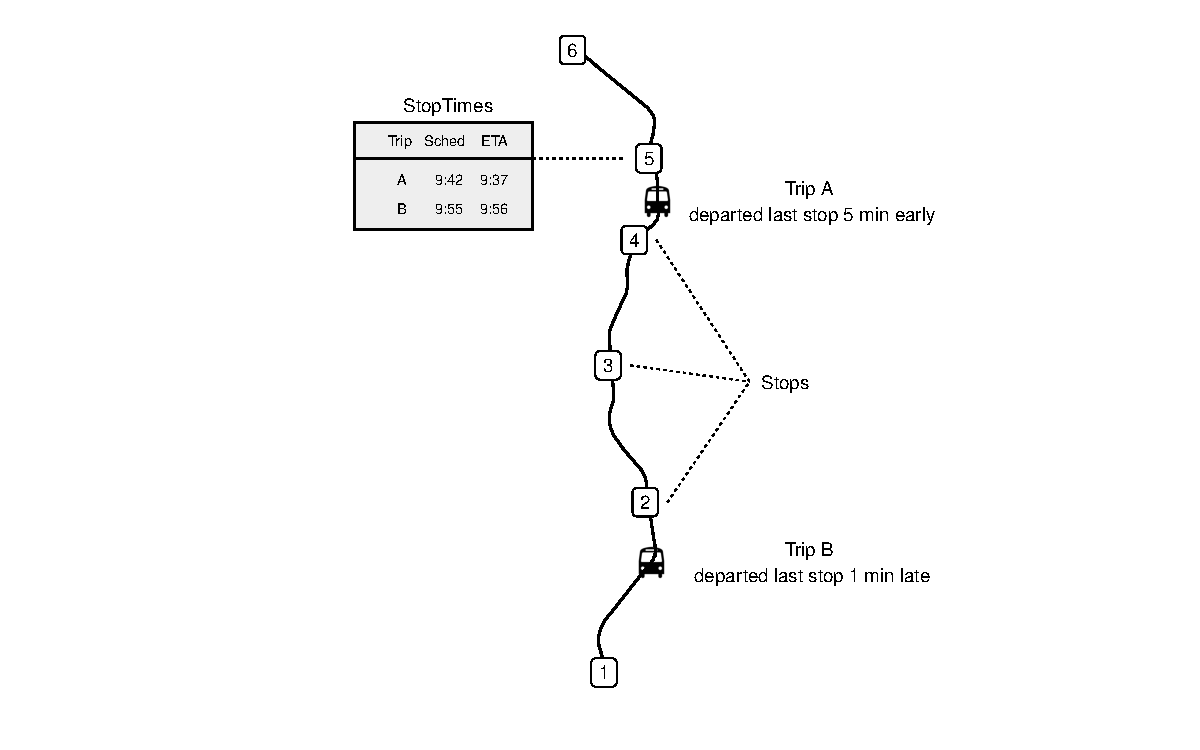
\includegraphics[width=\textwidth]{figure/gtfs_nw-1} 

}

\caption[The main components of a GTFS feed]{The main components of a GTFS feed for a single \emph{route} with two \emph{trips} (A and B) travelling along a \emph{shape} path. The numbered squares represent \emph{stops}, and the scheduled arrival times of each trip at stop 5 are displayed in the \emph{stop times} box.}\label{fig:gtfs_nw}
\end{figure}


\end{knitrout}



Transport providers typically distribute static \GTFS{} data in plain text files, one for each of the components (such as \verb+routes.csv+ and \verb+trips.csv+). Often these are available to download as a single ZIP archive, so the data is easily loaded into a \emph{relational database}, which is described further in \cref{app:gtfs}. The \Rstats{} package developed as part of this work provides the \verb+create_gtfs()+ function to do this automatically:
\begin{knitrout}\small
\definecolor{shadecolor}{rgb}{1, 1, 1}\color{fgcolor}\begin{kframe}
\begin{alltt}
\hlkwd{library}\hlstd{(transitr)}
\hlstd{nw} \hlkwb{<-} \hlkwd{create_gtfs}\hlstd{(}\hlstr{"at_gtfs.zip"}\hlstd{,} \hlkwc{db} \hlstd{=} \hlstr{"at_gtfs.sqlite"}\hlstd{)}
\end{alltt}
\end{kframe}
\end{knitrout}


Within these separate files or tables, the data is stored as per \GTFS{}. Importantly, shapes are stored as sequences of coordinates that draw a path on a map, while stops are represented as a single coordinate marking the location of the bus stop. Stop times are stored in trip-stop pairs with one row for every stop of each trip, along with the scheduled arrival and departure times.\footnote{There are 732,184 rows in the stop times table for Auckland Transport!}



On its own, the static \GTFS{} information can be used like a printed timetable, allowing simple journey planning to take place. As such, it provides a ``fallback'' state in situations where no \rt{} information is available for a given trip: scheduled stop times can be thought of as \emph{prior information}, a core component of the Bayesian paradigm.



\subsection{Real-time GTFS}
\label{sec:gtfs_rt}

The real-time component of \GTFS{} is responsible for handling vehicle positions, trip updates (arrivals at and departures from stops), and service alerts (cancellations and stop closures, for example). Data is processed by a central server and then stored appropriately to enable quick access via \glspl{api}. There is, therefore, the additional need of a server that can handle vast numbers of \gls{api} requests. As such, only a subset of transport providers using \GTFS{} have also implemented the real-time component. Below we give a summary of these components, but further information is available on the \GTFS{} website.\footnote{See \url{https://developers.google.com/transit/gtfs-realtime/}.}


\subsubsection{Vehicle positions}
\label{sec:gtfs_rt_vehicle}

There are several key components to a vehicle position (in the context of \GTFS{}). The \emph{vehicle descriptor} includes information about the physical vehicle, while a \emph{trip descriptor} holds information about the trip being serviced. A \emph{timestamp} specifies exactly when the observation was made, and a \emph{position} contains the actual data, such as the \gls{gps} observation, as is demonstrated by the bus images in \cref{fig:gtfs_nw}.


The specification also allows for additional measurements, such as \emph{speed} or an \emph{odometer} reading. However, these were not available from \AT{} at the time this work was carried out, so they are not included in our application. It is well worth noting, however, that they could be integrated with minimal effort if they become available.


\subsubsection{Trip updates}
\label{sec:gtfs_rt_trip}

As vehicles equipped with \gls{avl} technology arrive at and depart from stops, information about their times of arrival and, most importantly, \emph{schedule adherence} is stored in trip updates. These also contain a \emph{trip descriptor}, as well as one or more \emph{stop time updates}. GTFS-realtime allows storing of stop time updates for all previously visited stops, as well as predictions for upcoming stops. However, Auckland Transport only stores the most recent update.


Each stop time update reports either the arrival or departure time and, where schedule information is available, the schedule adherence by way of an \emph{arrival} or \emph{departure delay} (in seconds). \Cref{fig:gtfs_nw} displays this information offset to the right of each bus location. The on-board \gls{avl} device is responsible for detecting these events, and they are not necessarily linked to the \gls{gps} position of the vehicle. In Auckland, each trip update also triggers a vehicle location update, but the coordinates are those of the \emph{stop}, not of the vehicle. This leads to some of the problems addressed in \cref{sec:realtime-data}.


In Auckland, the current delay is added to the scheduled arrival time, as shown on the \gls{dms} in \cref{fig:gtfs_nw}. We will certainly be discussing the issues associated with this method shortly, and indeed be making comparisons to it throughout the thesis.



\subsubsection{Service alerts}
\label{sec:gtfs_rt_alerts}

Less important for the current work, but essential for reliable \gls{rti}, \emph{service alerts} enable transit operators to modify the static \GTFS{} in real-time. So, when a trip is cancelled, they can send out a service alert announcing the cancellation,\footnote{Although they often don't.} which is then displayed to passengers as a ``C'' on the \gls{dms}. It is also possible to add trips, for example during special events, or to reroute trips around stop closures, but this is beyond the scope of our work.



\subsection{Accessing \rt{} data (API)}
\label{sec:gtfs_rt_api}

Distributing vehicle locations, trip updates, and service alerts to passengers quickly and usefully requires more than just a \gls{dms} at bus stops. Personal mobile devices have revolutionised the way we live our lives, and developers are continually creating new applications to assist with everyday activities. Included in these are transit applications, which are capable of conveying real-time \GTFS{} data to passengers.


The most common method of distributing real-time data is via an \gls{api}. This is, in simple terms, a fixed web address from which developers can request a data file---either \prog{JSON} or, in the case of some \GTFS{} systems, \prog{protobuf}\footnote{See \url{https://developers.google.com/protocol-buffers}}---which can then be parsed and displayed to users. Usually, developers need to register for an \emph{\gls{api} key} which helps to control server demand by limiting the number of requests a user can make, or control access to specific data. The \pkg{transitr} package includes the ability to connect to a \GTFS{}-based \gls{api} easily:
\begin{knitrout}\small
\definecolor{shadecolor}{rgb}{1, 1, 1}\color{fgcolor}\begin{kframe}
\begin{alltt}
\hlstd{url} \hlkwb{<-} \hlstr{"https://api.at.govt.nz/v2/public/realtime/vehiclelocations"}
\hlstd{nw} \hlkwb{<-} \hlkwd{load_gtfs}\hlstd{(}\hlstr{"at_gtfs.sqlite"}\hlstd{)} \hlopt
    \hlkwd{realtime_feed}\hlstd{(url)} \hlopt
    \hlkwd{with_headers}\hlstd{(}
        \hlcom{# this varies by provider}
        \hlstr{"Ocp-Apim-Subscription-Key"} \hlstd{=} \hlkwd{Sys.getenv}\hlstd{(}\hlstr{'APIKEY'}\hlstd{)}
    \hlstd{)}
\end{alltt}
\end{kframe}
\end{knitrout}

\section{Charactersitics of real-time transit data}
\label{sec:realtime-data}

There are a range of \gls{avl} technologies which allow transit vehicles to report their locations in real-time. The most common of these is now the \gls{gps}, which provides the longitude and latitude of the vehicle. In the simplest of deployments, each vehicle reports its location to a central server at a fixed time interval. The server then collates the reports from all buses in the fleet and makes them available via an \gls{api}.


Another type of real-time data available to us is arrival and departure information at bus stops. When a vehicle arrives at or departs from a stop,\footnote{Or thinks it does, see \cref{sec:vp_data}.} it reports to the server which stop it is at along with its time of arrival or departure. The server then computes the delay (the time between actual and scheduled arrival or departure), collates the data from multiple vehicles, and also makes these available through an \gls{api}.


\Gls{rti} can be displayed in one of two ways. \Gls{gps} positions are displayed on a map accessed through a mobile app, allowing commuters to see where their bus was when it last reported its location. For trip updates, the \emph{current delay} is added to the scheduled arrival time and displayed to commuters, usually as a \emph{time until arrival}, in minutes.\footnote{That is ``scheduled arrival time + delay - current time''.} The \gls{eta} can be displayed either on a mobile app or, more commonly, on a \gls{dms} at the stop.


What we have just described is, in fact, the entirety of \gls{rti} in Auckland and some other transit locations around the world. While at first it seems an adequate solution, discussion with just about any regular public transport user suggests otherwise. The reasons for this become apparent with a little scrutiny, which we will now uncover.


\subsection{Vehicle positions}
\label{sec:vp_data}

Every measurement of a data point comes with some associated error. In the case of \gls{gps} devices, this error is usually small with precision depending on the quality of the device. However, any device can succumb to several factors which may place the bus far from its expected path, the primary reason being buildings or other obstacles resulting in a poor signal \citep{Xinghao_2013,Mutambara_2000,Zhao_1997}. Surprisingly, however, this is not the main issue with vehicle position data.


Object tracking has been well studied, and many algorithms exist for tracking an object through space using \gls{gps} observations. However, these usually take high-frequency observations (\citet{Gustafsson_2002} updated the car's location twice per second) which can generate an almost exact real-time estimate of the object's actual position.


Many examples of real-time object tracking exist, but the most relatable to most readers will be in their pocket. When getting directions from your phone, the maps application requests the user's phone's location continuously, providing the exact location with a second or less of delay. However, have you ever been driving along, following directions, and accidentally missed the turn-off? Often, the maps application will show you as \emph{on course} for several seconds until it realises that you have well and truly gone off-track and reroutes you. This is an example of a real-time position tracking algorithm that is attempting to follow the device's location while simultaneously accounting for inherent noise in the measurements. When the driver first goes off track, the algorithm assumes this is a measurement error and assumes the vehicle is on course. Eventually, the error becomes large and consistent enough that the model stops assuming the driver is following the planned route.


With real-time transit data, the frequency of observations is vastly reduced, with observations obtained with anything from ten seconds to a minute (or more) between them. This makes it very difficult to estimate the vehicle's exact location. On receiving a vehicle position that seems incorrect, we must wait until we receive the next observation to determine if it was the result of a bad measurement or a real event.


Another major complication with the Auckland Transport vehicle data is that vehicles often report their location when arriving at or departing from a bus stop. However, instead of reporting their \gls{gps} location as measured from the \gls{gps} device, they report the location of the bus stop itself, which is known exactly. So, what happens when the bus approaches a bus stop at speed, only to come to a halt at an intersection 100~m before hand? The vehicle's \gls{avl} system continues predicting the trajectory and places the vehicle at the bus stop before it actually arrives. This triggers a trip update (section~\ref{sec:tu_data}), which itself produces a vehicle position update \emph{at the bus stop}. However, a passenger standing at the stop will see the bus sitting at the lights even though the \gls{dms} displays the bus as having arrived. For the passenger waiting at this stop, this is of no concern, as they can see the bus and have no need for real-time data. For passengers farther down the line, however, this can have some frustrating implications.

Another related phenomenon exists in which the bus may appear to go backwards according to the sequence of \gps{} coordinates, discussed in detail in \cref{sec:data_issues}. The main consequence of this problem is that within the data processing component of our application, we check for vehicle position updates associated with trip updates and remove them (that is, we use the trip update and not the vehicle position).\footnote{This seems straightforward, but was frustrating until identified.}




\subsection{Trip updates}
\label{sec:tu_data}

As alluded to earlier, trip updates are prone to measurement error. Without human intervention, it is challenging for the \gls{gps} tracking system on the bus to determine exactly when the bus arrives at or leaves a bus stop. In situations like the one described above, the arrival time may be reported before the bus arrives, resulting in a premature arrival time and, more importantly, \emph{a reduced delay}. Traffic lights may hold up a bus for a minute (or more), so the bus may, for argument sake, appear to arrive precisely on time with a delay of zero minutes. The result of this is the propagation of the current delay to all future stops, which then display an \gls{eta} that matches the scheduled arrival time. However, two minutes later, after the bus has finally arrived at the stop, dropped off and picked up passengers, it departs, triggering another trip update. The delay, now two minutes, is propagated to upcoming stops. Passengers waiting at these stops see the \gls{eta} jump suddenly by two minutes, as demonstrated in \cref{fig:tu_eta_jump}, leading inevitably to much frustration for passengers.

\begin{knitrout}\small
\definecolor{shadecolor}{rgb}{0.969, 0.969, 0.969}\color{fgcolor}\begin{figure}

{\centering 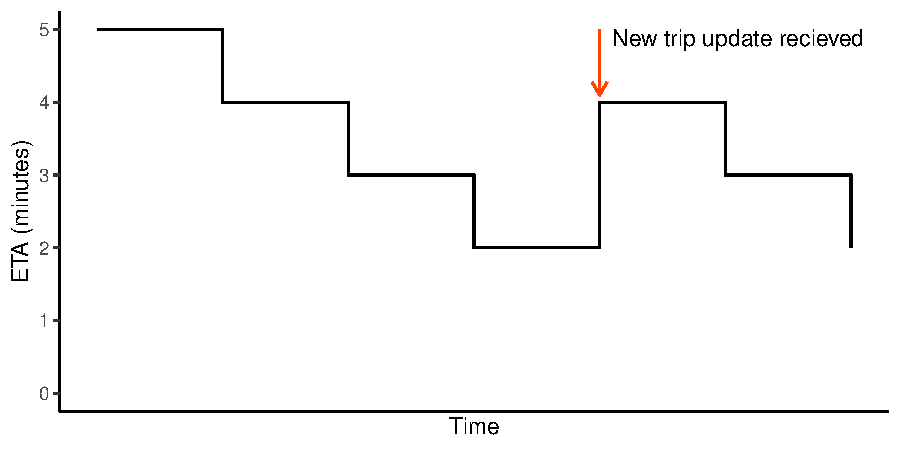
\includegraphics[width=.8\textwidth]{figure/tu_eta_jump-1} 

}

\caption[ETAs as percieved by passengers under the current system]{The current system displays \glspl{eta} to passengers as integer minutes which decrease over time. When new data is recieved (marked by an arrow) the \gls{eta} is updated, which may result in a sudden ``jump'', as demonstrated.}\label{fig:tu_eta_jump}
\end{figure}


\end{knitrout}


The reverse can also occur, for example, if for some reason the bus reports its arrival or departure late. However, more prevalent is that the update is skipped altogether, so a bus that was five minutes behind schedule has made up several minutes and arrives at the bus stop while the \gls{dms} still shows it as being two minutes away. At first, this may seem like a good thing: passengers at the stop have a shorter wait. Other passengers making their timely way to the bus, however, may have to sprint or miss the bus altogether, which is not ideal.


The main repercussion of the described issues is that arrival and departure time data become very noisy and difficult to trust. They do, however, provide a lot of information without which it would be challenging to infer the trajectory of a bus between stops---which is the primary aim of this part of our work. We discuss this further in \cref{sec:pf-likelihood} when I present the likelihood function.



\section{Constructing a network from GTFS data}
\label{sec:route-segments}

In \cref{sec:literature}, I reported how arrival time prediction is greatly improved when data from multiple routes is combined to estimate traffic conditions \citep{Yu_2011}. However, many of these applications were specific to a certain set of routes, or used external information (such as automatic toll readers and taxis) to get \rt{} traffic information. We wanted to develop a \emph{simpler}, \emph{more generalised} approach using solely \GTFS{} data (stops and shapes) to construct a network of non-overlapping\footnote{Except of course reverse directions.} road segments. The network should consist of \emph{nodes} (which could be intersections or bus stops) connected by \emph{edges}, or road segments, which is similar to the structure used by \citet{Celan_2017,Vuurstaek_2018}.


The main goal of the network is to detect where any two routes overlap, even partially. There are several possible approaches to this, but the simplest is to look at common subsequences of bus stops. Of course, stops do not make optimal node locations because routes do not diverge \emph{physically} at stops---that would require locating \emph{intersections}. However, due to difficulties in finding intersections from either the \gls{gtfs} data or outside information, we opted to use bus stops for this work. \Cref{fig:gtfs_route_network} shows a simple route diagram with several overlapping routes. We see that each link between stops is common across routes, but routes that merge at intersections do not merge in the network until they reach a common stop.


\begin{knitrout}\small
\definecolor{shadecolor}{rgb}{1, 1, 1}\color{fgcolor}\begin{figure}

{\centering 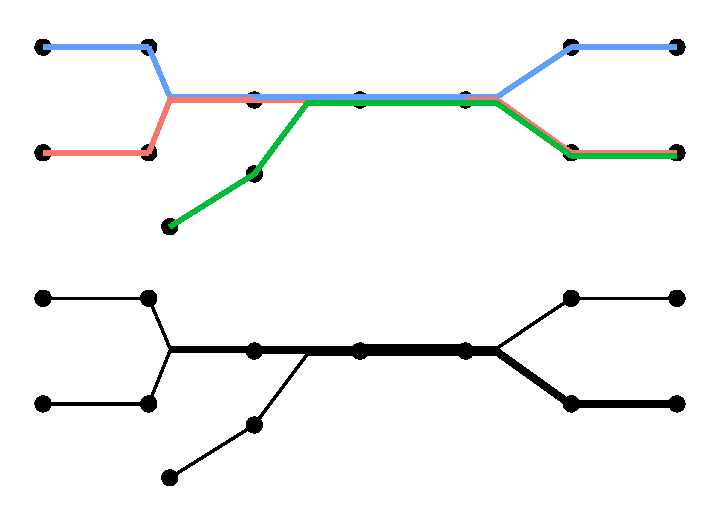
\includegraphics[width=0.6\textwidth]{figure/gtfs_route_network-1} 

}

\caption[Simplified network diagram with road segments constructed from stop sequences]{Simplified network diagram with road segments constructed from stop sequences. Top: routes are coloured individually. Bottom: road segments are sized by the number of associated routes.}\label{fig:gtfs_route_network}
\end{figure}


\end{knitrout}





One other issue with \AT{}'s \GTFS{} data is that all object IDs are \emph{versioned}. That is, instead of a route having an ID of \verb+02702+, the date and version number are appended to it: \verb+02702-20190806160740_v82.21+. This is the same for the IDs of trips, shapes, and stops, making it challenging to transfer existing segments based on stops from previous versions of the \gls{api} and requiring an additional step to remove the version information from the raw data.


The algorithm we implemented uses only bus stops but can extend to intersections, if available. Each stop along a route is assessed to see if any nodes already exist in that location to avoid the versioning issue mentioned above. If so, the route is assigned the existing node; otherwise, a new node is created and assigned instead. Road segments are defined by unique one-way connections between two stops: there can only be one segment going from node $A$ to node $B$ (the reverse is considered a different segment). The network is constructed by the \pkg{transitr} package's \verb+construct()+ function:
\begin{knitrout}\small
\definecolor{shadecolor}{rgb}{1, 1, 1}\color{fgcolor}\begin{kframe}
\begin{alltt}
\hlkwd{library}\hlstd{(transitr)}
\hlstd{nw} \hlkwb{<-} \hlkwd{load_gtfs}\hlstd{(}\hlstr{"at_gtfs.sqlite"}\hlstd{)} \hlopt \hlkwd{construct}\hlstd{()}
\hlstd{transitr}\hlopt{:::}\hlkwd{load_road_segments}\hlstd{(nw)} \hlopt \hlkwd{head}\hlstd{()}
\end{alltt}
\begin{verbatim}
##   road_segment_id node_from node_to    length
## 1               1      5414     537  485.6548
## 2               2       537    3987  196.5567
## 3               3      3987    7265  567.0883
## 4               4      7265    1255 1049.0181
## 5               5      1255    4099  682.5452
## 6               6      4099    3436  535.0515
\end{verbatim}
\end{kframe}
\end{knitrout}

\section{Recursive Bayesian models}
\label{sec:recursive-bayes}

The most challenging problem we face in this application is its \rt{} nature. Vehicle's report their current location, from which we want to estimate road speeds to predict arrival times, all within no more than 30~seconds. Fortunately, a certain class of models suit themselves well to \rt{} applications, and are indeed used in many vehicle tracking and robotics applications \citep{Anderson_1979,Gustafsson_2002,Mutambara_2000}: \glspl{rbm}, sometimes referred to a \emph{sequential Bayesian estimation}.


In a typical analysis, data $\mat{Y}$ would be stored in an $n\times k$ matrix corresponding to $k$ measurements of $n$ variables over time. Then Bayes' rule is used to estimate the posterior distribution of an $m\times k$ matrix of parameters $\mat{X}$ all at once,
\begin{equation}
\label{eq:bayes}
p(\mat{X}\cond{}\mat{Y}) =
\frac{
    p(\mat{X})
    p(\mat{Y}\cond{}\mat{X})
}{
    p(\mat{Y})
},
\end{equation}
using, for example, \agls{mcmc} algorithm. This is usually a computationally intensive procedure and takes much longer than 30~seconds to converge.


In a real-time application, the columns of $\mat{Y}$ are observed sequentially, so that at time $t_k$ we have observed
\begin{equation}
\label{eq:bayes_y_vector}
\mat{Y} = \boldsymbol{y}_{1:k} = [\boldsymbol{y}_1,\cdots,\boldsymbol{y}_k],
\end{equation}
to estimate
\begin{equation}
\label{eq:bayes_x_vector}
\mat{X} = \bx_{0:k} = [\boldsymbol{x}_0,\cdots,\boldsymbol{x}_k],
\end{equation}
where $\boldsymbol{x}_0$ is the \emph{initial state} of the object. Rather than refitting the full model, as would be necessary when using \gls{mcmc}, \gls{rbe} allows us to combine the previous \emph{posterior estimate} of the state with the new information.

\Glspl{rbm} make two general assumptions. The first is that $\boldsymbol{x}$ follows a Markov process such that the state at time $t_k$ depends only upon the state at time $t_{k-1}$:
\begin{equation}
\label{eq:rbe_markov}
p(\boldsymbol{x}_k \cond{} \boldsymbol{x}_{0:k-1}) =
p(\boldsymbol{x}_k \cond{} \boldsymbol{x}_{k-1}).
\end{equation}
The joint distribution of the underlying state parameters is therefore
\begin{equation}
\label{eq:rbe_joint_x}
\begin{split}
p(\bx_{0:k})
&= p(\bx_0)p(\bx_1\cond{}\bx_0)p(\bx_2\cond{}\bx_{0:1})\cdots
p(\bx_{k}\cond{}\bx_{0:k-1}) \\
&= p(\bx_0)p(\bx_1\cond{}\bx_0)p(\bx_2\cond{}\bx_1)\cdots p(\bx_k\cond{}\bx_{k-1}) \\
&= p(\bx_0)\prod_{i=1}^k p(\bx_i\cond{}\bx_{i-1}).
\end{split}
\end{equation}

The second assumption is that the observations $\boldsymbol{y}_k$ of the state depend only on the current state and are independent of one another:
\begin{equation}
\label{eq:rbe_obs}
p(\boldsymbol{y}_k \cond{} \boldsymbol{x}_{0:k}, \boldsymbol{y}_{0:k-1}) =
p(\boldsymbol{y}_k \cond{} \boldsymbol{x}_{k}).
\end{equation}
Thus, the data has joint likelihood
\begin{equation}
\label{eq:rbe_joint_lh}
\begin{split}
p(\boldsymbol{y}_{1:k}\cond{}\bx_{0:k})
&= p(\boldsymbol{y}_1\cond{}\bx_{0:1})\cdots p(\boldsymbol{y}_k\cond{}\bx_{0:k}) \\
&= p(\boldsymbol{y}_1\cond{}\bx_1)\cdots p(\boldsymbol{y}_k\cond{}\bx_k) \\
&= \prod_{i=1}^k p(\boldsymbol{y}_i\cond{}\bx_i)
\end{split}
\end{equation}
and marginal distribution
\begin{equation}
\label{eq:rbe_marginal_y}
p(\boldsymbol{y}_{1:k}) = p(\boldsymbol{y}_1)\cdots p(\boldsymbol{y}_k)
= \prod_{i=1}^k p(\boldsymbol{y}_i).
\end{equation}



We now express the posterior distribution $p(\bx_{0:k}\cond{}\boldsymbol{y}_{1:k})$ using \cref{eq:bayes} along with \cref{eq:rbe_joint_x,eq:rbe_joint_lh,eq:rbe_marginal_y} as
\begin{equation}
\label{eq:rbe_posterior}
\begin{split}
p(\bx_{0:k}\cond{}\boldsymbol{y}_{1:k})
&= \frac{p(\bx_{0:k})p(\boldsymbol{y}_{1:k}\cond{}\bx_{0:k})}{p(\boldsymbol{y}_{1:k})} \\
&= \frac{
    p(\bx_0)\prod_{i=1}^k p(\bx_i) \cdot
    \prod_{i=1}^k p(\boldsymbol{y}_i\cond{}\bx_i)
}{
    \prod_{i=1}^k p(\boldsymbol{y}_i)
} \\
&= p(\bx_0)\prod_{i=1}^k
\frac{
    p(\bx_i) p(\boldsymbol{y}_i\cond{}\bx_i)
}{
    p(\boldsymbol{y}_i)
}.
\end{split}
\end{equation}
However, we can substitute the first $k-1$ terms in \cref{eq:rbe_posterior} to obtain the following recursive representation:
\begin{equation}
\label{eq:rbe_posterior_recursive}
p(\bx_{0:{k}}\cond{}\boldsymbol{y}_{1:k})
= p(\bx_{0:k-1}\cond{}\boldsymbol{y}_{1:k-1})
\frac{
    p(\bx_{k}) p(\boldsymbol{y}_{k}\cond{}\bx_{k})
}{
    p(\boldsymbol{y}_{k})
}.
\end{equation}
Here, the posterior distribution from the previous time step is used as a \emph{prior} for the next, and so it \emph{recursively} (or \emph{sequentially}) updates the state estimate as new data are observed, making \glspl{rbm} ideal for real-time applications.


There are several types of \glspl{rbe} which consist of two main steps: \emph{predict} and \emph{update}. In the prediction step, the algorithm uses a \emph{transition function} $f$ (or matrix $\mat{F}$) to predict the new state based only upon the current state (\cref{eq:rbe_markov}), while the \emph{update} step incorporates the data to adjust the estimate using a \emph{measurement function} $h$ (or matrix $\mat{H}$) describing the relationship between $x$ and $y$ (\cref{eq:rbe_obs}). These can be expressed by the following model equations:
\begin{equation}
\label{eq:rbe_model}
\begin{split}
\bx_k &= f(\bx_{k-1}, \boldsymbol{w}_k) \\
\boldsymbol{y}_k &= h(\bx_k) + \boldsymbol{v}_k
\end{split}.
\end{equation}
The additional parameters $\boldsymbol{w}_k$ and $\boldsymbol{v}_k$ represent \emph{system noise} and \emph{measurement error}, respectively. The choice of $f$, $h$, and the distributions for the error terms depends on the choice of model. We now discuss two types of \gls{rbe} used throughout this thesis: the \kf{} and the \pf{}.


\subsection{\kf{}}
\label{sec:kf}

Commonly used in vehicle tracking applications, the \kf{} is a very fast, simple estimation method \citep{Anderson_1979} that assumes Gaussian errors and represents the state using a multivariate Normal random variable with length $m$ mean vector and $m\times x$ covariance matrix
\begin{equation}
\label{eq:kf_estimators}
\hat\bx_{k|k} = \E{\bx_k | \boldsymbol{y}_{1:k}}
\quad\text{and}\quad
\mat{P}_{k|k} = \Var{\bx_k | \boldsymbol{y}_{1:k}},
\end{equation}
respectively. A \kf{} implementation requires an $m\times m$ \emph{transition matrix}, $\mat{F}_k$, which defines the relationship between states at time $t_{k-1}$ and $t_k$, and an $n\times m$ \emph{measurement matrix}, $\mat{H}_k$, defining the relationship between $\boldsymbol{y}$, a length $n$ vector, and $\bx$, a length $m$ vector.


The \kf{} version of the model presented in \cref{eq:rbe_model} is
\begin{equation}
\label{eq:kf_model}
\begin{split}
\bx_k &= \mat{F}_k\bx_{k-1} + \boldsymbol{w}_k \\
\boldsymbol{y}_k &= \mat{H}_k\bx_k + \boldsymbol{v}_k
\end{split},
\end{equation}
where $\boldsymbol{w}_k$ and $\boldsymbol{v}_k$ are Normal random variables with mean zero and covariance matrices $\mat{Q}_k$ and $\mat{R}_k$, respectively. The $m\times m$ covariance matrix $\mat{Q}_k$ represents the system noise at time $t_k$, which is defined as the rate of change of the variance of process noise \citep{Cathey_2003}. Measurement error is expressed by the $n\times n$ covariance matrix $\mat{R}_k$.

The \kf{} is implemented through two sets of equations. First is the prediction step, in which the current state (represented by the mean vector and covariance matrix) is predicted based solely on the previous state:
\begin{equation}
\label{eq:ch2:kf_predict}
\begin{split}
\hat\bx_{k|k-1} = \E{\bx_k | \bx_{k-1}}
    &= \mat{F}_k \hat\bx_{k-1|k-1} \\
\mat{P}_{k|k-1} = \Var{\bx_k | \bx_{k-1}}
    &= \mat{F}_k \mat{P}_{k-1|k-1} \mat{F}_k^\top + \mat{Q}_k
\end{split}
\end{equation}
Next, the update step uses the observation $\boldsymbol{y}_k$ to adjust the predicted state using the following set of equations, which are effectively taking a ratio of the state and measurement uncertainties:
\begin{equation}
\label{eq:ch2:kf_update}
\begin{split}
\bz_k &= \boldsymbol{y}_k - \mat{H}_k \hat\bx_{k|k-1} \\
\mat{S}_k &= \mat{R}_k + \mat{H}_k \mat{P}_{k|k-1} \mat{H}_k^\top \\
\mat{K}_k &= \mat{P}_{k|k-1} \mat{H}_k^\top \mat{S}_k^{-1} \\
\hat\bx_{k|k} &= \hat\bx_{k|k-1} + \mat{K}_k \bz_k \\
\mat{P}_{k|k} &= (\mat{I} - \mat{K}_k \mat{H}_k) \mat{P}_{k|k-1}
    (\mat{I} - \mat{K}_k \mat{H}_k)^\top + \mat{K}_k \mat{R}_k \mat{K}_k^\top.
\end{split}
\end{equation}


The simplicity of the \kf{} means that, so long as the number of parameters $m$ is small, states can be estimated quickly with minimal processing demand. This simplicity, together with the fact that it provides an exact solution for the multivariate Normal state space model \citep{Anderson_1979}, makes the \kf{} a strong contender for real-time applications. However, it also makes several strong assumptions about the shape of the parameter distributions and is limited to linear relationships between states and measurements since these must be expressed in matrix form.



\subsection{Particle filter}
\label{sec:pf}

Another framework we use is the \pf{}, a more generalised, numerical approach to recursive Bayesian modelling \citep{Gordon_1993}. The state is approximated by a sample of $\Np$ particles, each of which is an independent point estimate of the state, $\bx\vi_k$, with a weight $w\vi \geq 0$ and $\sum_i w\vi = 1$. The state estimate is expressed using the Dirac delta measure $\dirac$ (see \cref{app:dirac-delta-measure} for details), such that
\begin{equation}
\label{eq:pf_state}
p(\bx_{k-1} | \boldsymbol{y}_{1:k-1}) \approx
\sum_{i=1}^\Np w\vi_{k-1} \DiracMeasure{\bx\vi_{k-1}}{\bx_{k-1}}.
\end{equation}

One advantage of the \pf{} is that we are no longer constrained in the choice of transition function, $f$, or the error distribution. Instead of working with the mean and variance of the state (as is the case with the \kf{}) we work with \emph{independent point estimates} which each represent a plausible state. In \cref{cha:vehicle_model} I use a Normal random variable for system noise, but this could be any appropriate distribution (for example a Cauchy if heavier tails are necessary). The state prediction step is carried out independently on each particle,
\begin{equation}
\label{eq:ch2:pf_predict_particle}
\bx\vi_k = f\left(\bx\vi_{k-1}, \boldsymbol{v}\vi_k\right),
\quad
\boldsymbol{v}\vi_k \sim \Normal{\boldsymbol{0}}{\mat{Q}_k}.
\end{equation}
The prior-predictive distribution of the state, using the Dirac delta measure, is given by
\begin{equation}
\label{eq:ch2:pf_predict_state}
p(\bx_k | \bx_{k-1}) \approx
\sum_{i=1}^\Np w\vi_{k-1} \DiracMeasure{\bx\vi_k}{\bx_k}.
\end{equation}


Next, the state is updated to account for the observation using the likelihood function directly. The particles are reweighted and normalised,
\begin{equation}
\label{eq:pf_reweight}
w\vi_k =
\frac{
    w\vi_{k-1} p(\boldsymbol{y}_k | \bx\vi_k)
}{
    \sum_{j=1}^\Np w\vi_{k-1} p(\boldsymbol{y}_k | \bx\vi[j]_k)
},
\end{equation}
which yields the final posterior distribution of the state,
\begin{equation}
\label{eq:pf_state_post}
p(\bx_{k} | \boldsymbol{y}_{1:k}) \approx
\sum_{i=1}^\Np w\vi_{k} \DiracMeasure{\bx\vi_{k}}{\bx_{k}}.
\end{equation}


Over time, many of the particle weights will go to zero as they disperse due to the system noise \citep{Doucet_2000}. This leaves only a few particles contributing to the state, which, if none end near the actual vehicle location, will result in all vehicles having likelihoods close to zero. To prevent this situation of particle filter \emph{degeneration}, we perform \emph{importance resampling} (a weighted bootstrap) in which particles are sampled, with replacement, according to their weight. Afterwards, particle weights are reset to $N^{-1}$.

\citet{Doucet_2000} describe the use of the \emph{effective sample size},
\begin{equation}
    \label{eq:Neff}
    N_{\text{eff}} \approx \frac{1}{\sum_{i=1}^N (w_k\vi)^2},
\end{equation}
which provides an estimate of how varied the particles are: if too few particles contain most of the weight, resampling should occur. This is similar to the Metropolis-Hasting's proposal and acceptance steps: we propose a sample of state estimates and reject those that are not plausible given the data. If the system noise (proposal distribution) is small, then more particles will be ``accepted'', but we may not propose sufficient trajectories. Conversely, if the noise is too large, then there will be many ``rejections'', reducing the variety of particles (small $N_\text{eff}$).

Another advantage of the \pf{} is its generality. As we discuss in \cref{sec:vehicle_model}, we can easily construct a transition function to describe a complex system, as well as define a likelihood function that accurately represents the relationship between observed and unobserved states.

The main disadvantage is, of course, that the computational demand is high, as each particle is transitioned independently, and resampling can be slow for large $\Np$, having order $\mathcal{O}(\Np\log\Np)$ in the \prog{C++} algorithm we use. However, as we discuss in the next chapter, the advantages far outweigh the additional computational demands of the \pf{}, which can be minimised if implemented carefully.




\section{\Rt{} implementation in Rcpp}
\label{sec:rt-implementation}

In \cref{sec:gtfs} I introduced the \Rstats{} package \pkg{transitr}, which loads a \GTFS{} database and connects to a real-time \gls{api}. The advantage of \Rstats{} \citep{rcore} is its superior ability for processing data of various forms through additional packages, and provision an easy-to-use interface for users. However, when it comes to computational efficiency, \Cpp{} is the better choice. Fortunately, \Rstats{} offers an interface to \Cpp{} through the \pkg{Rcpp} package developed by \citet{Rcpp}. This gives us the speed and memory management capabilities of \Cpp{} from within \Rstats{}.

The general structure of our program has two parts. The first handles data collection from a transit provider and creation of the transit network (\cref{sec:route-segments}), all stored in an \prog{SQLite} database.\footnote{\url{https://www.sqlite.org/index.html}} Users can connect to a GTFS-realtime \gls{api}, as well as pass additional arguments to the generated \obj{gtfs} object, which are then forwarded onto the second part which runs purely within \Cpp{}.

Within the \Cpp{} component, there are two main phases: setup and modelling. During the setup phase, the GTFS database is loaded, and parameter values are established. A vector of \class{Vehicle} objects is initialized to contain the real-time vehicle states. The modelling phase consists of a single \verb+while+ loop which runs until the operating system sends the program a kill signal. It is inside this loop that all of the real-time modelling discussed throughout the remainder of this thesis occurs.

Within the program, we use \gls{oop} to represent objects---both static (routes and trips) and \rt{} (vehicles, road segments). These objects contain a lot of \emph{interdependence}; for example, a trip belongs to a route and vehicles services trips. Pointers are used in \Cpp{} to allow easy access to these relationships without any duplication of information. For example, the route number for a vehicle can be obtained as follows:
\begin{knitrout}\small
\definecolor{shadecolor}{rgb}{1, 1, 1}\color{fgcolor}\begin{kframe}
\noindent
\ttfamily
\hlstd{vehicle}\hlopt{.}\hlstd{}\hlkwd{trip\ }\hlstd{}\hlopt{(){-}$>$}\hlstd{}\hlkwd{route\ }\hlstd{}\hlopt{(){-}$>$}\hlstd{}\hlkwd{route\textunderscore short\textunderscore name\ }\hlstd{}\hlopt{();}\hlstd{}\hspace*{\fill}
\mbox{}
\normalfont
\end{kframe}
\end{knitrout}
As pointers are not fixed, the above example works even after the vehicle changes to another trip. In addition to retrieving information, pointers can be used to pass information between objects. Later in this thesis, vehicles are used to estimate traffic conditions along individual roads, and then forward these observations on to the appropriate road segment. First, note that a route follows a sequence of road segments, which are stored in \Cpp{} using a \verb+std::vector+ containing an ordered sequence of \class{RouteSegment} objects, each pointing to the appropriate \class{Segment}. Thus, once a vehicle completes travel along the segment with index \verb+si+, the observed average speed can be passed directly to the \class{Segment}:
\begin{knitrout}\small
\definecolor{shadecolor}{rgb}{1, 1, 1}\color{fgcolor}\begin{kframe}
\noindent
\ttfamily
\hlstd{vehicle}\hlopt{.}\hlstd{}\hlkwd{trip\ }\hlstd{}\hlopt{(){-}$>$}\hlstd{}\hlkwd{route\ }\hlstd{}\hlopt{()}\hspace*{\fill}\\
\hlstd{}\hlstd{\ \ \ \ }\hlstd{}\hlopt{{-}$>$}\hlstd{}\hlkwd{segments\ }\hlstd{}\hlopt{().}\hlstd{}\hlkwd{at\ }\hlstd{}\hlopt{(}\hlstd{si}\hlopt{){-}$>$}\hlstd{}\hlkwd{segment\ }\hlstd{}\hlopt{()}\hspace*{\fill}\\
\hlstd{}\hlstd{\ \ \ \ }\hlstd{}\hlopt{{-}$>$}\hlstd{}\hlkwd{push\textunderscore data\ }\hlstd{}\hlopt{(}\hlstd{speed}\hlopt{,\ }\hlstd{uncertainty}\hlopt{);}\hlstd{}\hspace*{\fill}
\mbox{}
\normalfont
\end{kframe}
\end{knitrout}
\noindent
This data is then handled by the \class{Segment} object (described later in \cref{cha:network_model}).

The main issue with pointers is that, if an object is deleted or moved, a pointer may no longer point to the appropriate object, resulting in a \emph{segmentation fault} and crashing the program at runtime. However, with care, and by checking a pointer is valid before using it, it is possible to avoid such problems. For example, the above would be better written as follows.
\begin{knitrout}\small
\definecolor{shadecolor}{rgb}{1, 1, 1}\color{fgcolor}\begin{kframe}
\noindent
\ttfamily
\hlstd{Trip}\hlopt{{*}\ }\hlstd{trip\ }\hlopt{=\ }\hlstd{vehicle}\hlopt{.}\hlstd{}\hlkwd{trip\ }\hlstd{}\hlopt{();}\hspace*{\fill}\\
\hlstd{}\hlkwa{if\ }\hlstd{}\hlopt{(}\hlstd{trip\ }\hlopt{==\ }\hlstd{}\hlkwc{nullptr}\hlstd{}\hlopt{)\ }\hlstd{}\hlkwa{return}\hlstd{}\hlopt{();}\hspace*{\fill}\\
\hlstd{Route}\hlopt{{*}\ }\hlstd{route\ }\hlopt{=\ }\hlstd{trip}\hlopt{{-}$>$}\hlstd{}\hlkwd{route\ }\hlstd{}\hlopt{();}\hspace*{\fill}\\
\hlstd{}\hlkwa{if\ }\hlstd{}\hlopt{(}\hlstd{route\ }\hlopt{==\ }\hlstd{}\hlkwc{nullptr}\hlstd{}\hlopt{)\ }\hlstd{}\hlkwa{return}\hlstd{}\hlopt{();}\hspace*{\fill}\\
\hlstd{}\hlkwa{if\ }\hlstd{}\hlopt{(}\hlstd{route}\hlopt{{-}$>$}\hlstd{segments}\hlopt{.}\hlstd{}\hlkwd{size\ }\hlstd{}\hlopt{()\ $<$=\ }\hlstd{index}\hlopt{)\ }\hlstd{}\hlkwa{return\ }\hlstd{}\hlopt{();}\hspace*{\fill}\\
\hlstd{Segment}\hlopt{{*}\ }\hlstd{segment\ }\hlopt{=\ }\hlstd{route}\hlopt{{-}$>$}\hlstd{segments}\hlopt{.}\hlstd{}\hlkwd{at\ }\hlstd{}\hlopt{(}\hlstd{index}\hlopt{){-}$>$}\hlstd{}\hlkwd{segment\ }\hlstd{}\hlopt{();}\hspace*{\fill}\\
\hlstd{}\hlkwa{if\ }\hlstd{}\hlopt{(}\hlstd{segment\ }\hlopt{==\ }\hlstd{}\hlkwc{nullptr}\hlstd{}\hlopt{)\ }\hlstd{}\hlkwa{return\ }\hlstd{}\hlopt{();}\hspace*{\fill}\\
\hlstd{segment}\hlopt{{-}$>$}\hlstd{}\hlkwd{push\textunderscore data\ }\hlstd{}\hlopt{(}\hlstd{speed}\hlopt{,\ }\hlstd{uncertainty}\hlopt{);}\hlstd{}\hspace*{\fill}
\mbox{}
\normalfont
\end{kframe}
\end{knitrout}

The last topic for this section is \emph{multithreading}, which is the process of using more than one CPU core to run the program with the assistance of \prog{OpenMP}.\footnote{https://www.openmp.org/} This requires that the program is \emph{threadsafe}, such that two independent cores will not adversely interact (for example by both trying to modify the same object). The simplest way around this is to perform read-only operations on common resources.

Sometimes, however, write operations are unavoidable, such as when passing data to road segments. \emph{Mutex locking} provides a simple way of ensuring that only one process can perform a specified task at a time. Continuing with the same example, if two vehicles traverse a road at the same time (which happens frequently), they will both want to push their observed speed observations to this same \class{Segment} object at the same time. To prevent errors, we create a lock at the beginning of the \verb+Segment::push_data ()+ method. Now when the first \class{Vehicle} calls \verb+push_data ()+, the \class{Segment} is ``locked'' until the method is complete (the data is processed and stored within the \class{Segment}). If a second \class{Vehicle} calls the method before the first has finished, it will find the \class{Segment} locked and the process will wait until the lock has been released before it can continue. This lets us parallelise the processing of vehicles to multiple cores, greatly speeding up iteration timings.

